


\begin{document}

This section details the experimental implementation of the two differential amplifiers, the resistively loaded and active loaded. The power supplies and analysis were implemented using the Digilent Analog Discovery kit.

The experimental circuit can be seen Figure \ref{fig:expercircuit}.

\begin{figure}[H]
	\begin{center}
		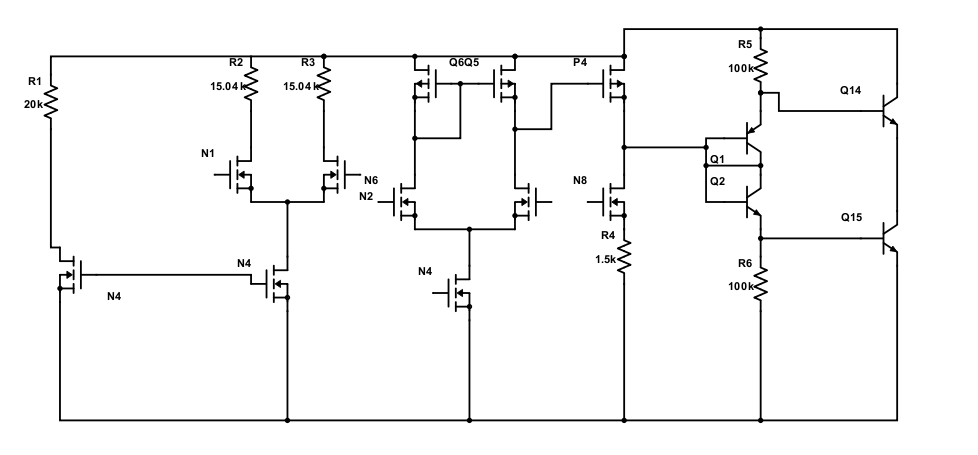
\includegraphics[scale=.40]{ExperimentalImplementation/task4.png}
		\caption{Experimental operational amplifier}
		\label{fig:expercircuit}
	\end{center}
\end{figure}
The 20 k$\Omega$ reference resistor achieved the desired current of 397 $\mu$A. The resistive loads were matched at 15.04 k$\Omega$.  This resulted in a difference of 30mV between the drains of the amplifying transistors. WORKING CIRCUIT STUFF GOES HERE.

\textbf{NOTE TO TA: The circuit stopped working during the final stages of testing over the weekend. As a result we currently have no graphs to put here as all attempts to rebuild
	have continued to lead to inoperable circuits. Apologies -- Lab group \#9.}
	
\end{document}


